\section{Data and Methods}
\label{sec:approach}

\subsection{Dataset Description}

We have used the following two datasets. The first and most important in our work is composed of information on loans and the credit of a large sample of Italian companies. The second reports balance sheet data of a large sub-sample of medium-large Italian companies.


\paragraph{Credit data.} 


It consists of a very large and high granular dataset of credit
information about Italian companies belonging to the Italian Central
Credit Register.
It is an information system on the debt
of the customers of the banks and financial companies supervised by the
Bank of Italy. Bank of Italy collects information on customers'
borrowings from the intermediaries and notifies them of the risk
position of each customer vis-à-vis the banking system.
By means of the Central Credit Register the Bank of Italy provides
intermediaries with a service intended to improve the quality of the
lending of the credit system and ultimately to enhance its stability.
The intermediaries report to the Bank of Italy on a monthly basis the
total amount of credit due from their customers: data information about
loans of 30,000 euro or more and non-performing loans of any amount.

Italian Central Credit Register has three main goals: a)
improve the process of assessing customer creditworthiness; b) to
raise the quality of credit granted by intermediaries; c) strengthen
the financial stability of the credit system. 




The crucial feature of this database is the high granularity of credit
information. To the best of our knowledge, Machine Learning techniques
have not yet been applied for the analysis of these database.
We used a overall credit dataset containing over 800,000 rows. Each row contain credit
data related to a single firm. For each firm the dataset contains about
20 different attributs; the most important are shown in the following
Table. We considered information on the dynamics
of credit to firm with quarterly frequency. The objective of the work is
to predict whether a company that at the time T was not in default
status in the following year will be classified in default. The complete
dataset used to make the predictions consists of credit information over
a period of five years from 2009 to 2014.
Central Credit Register data are not public.



\begin{figure}[H]
\flushleft
%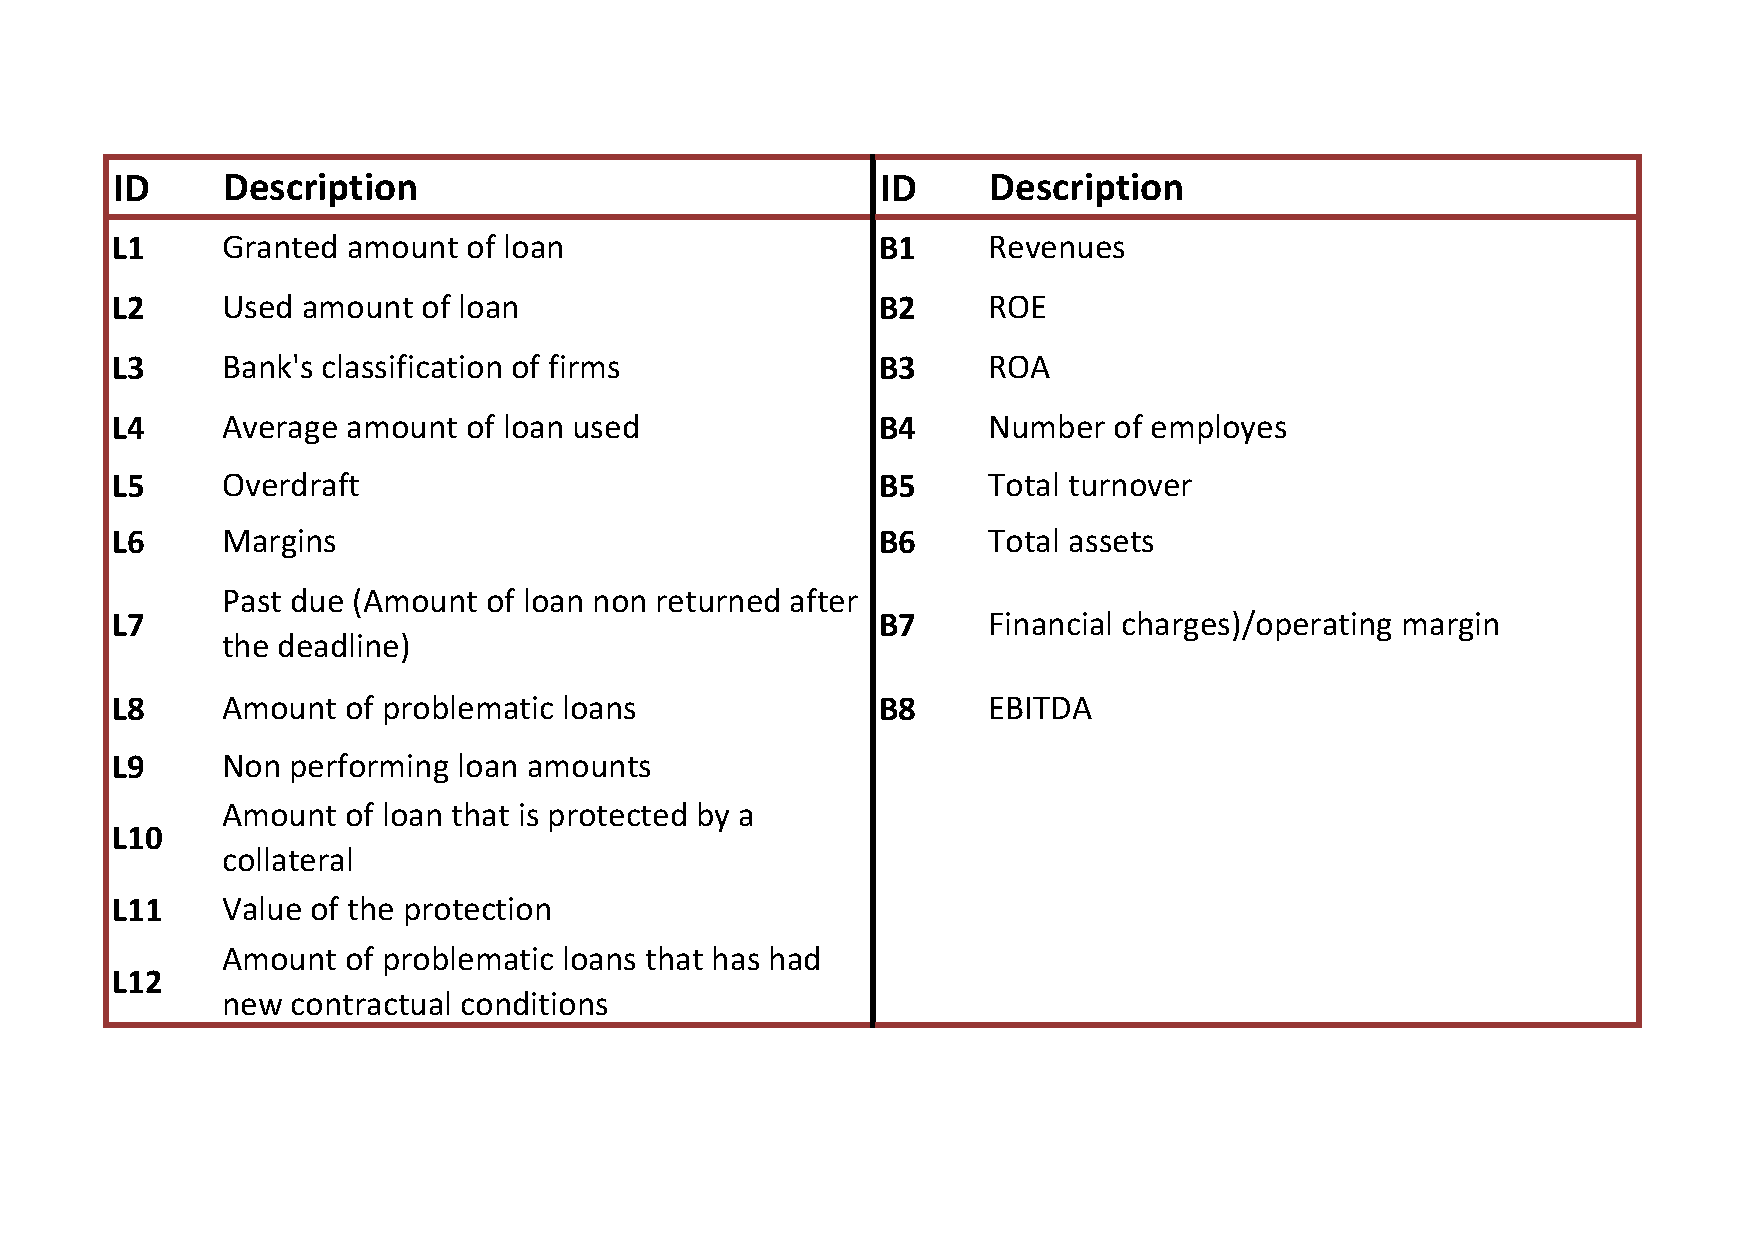
\includegraphics[width=180mm, height=80mm]{figs/Table_dataset.pdf}
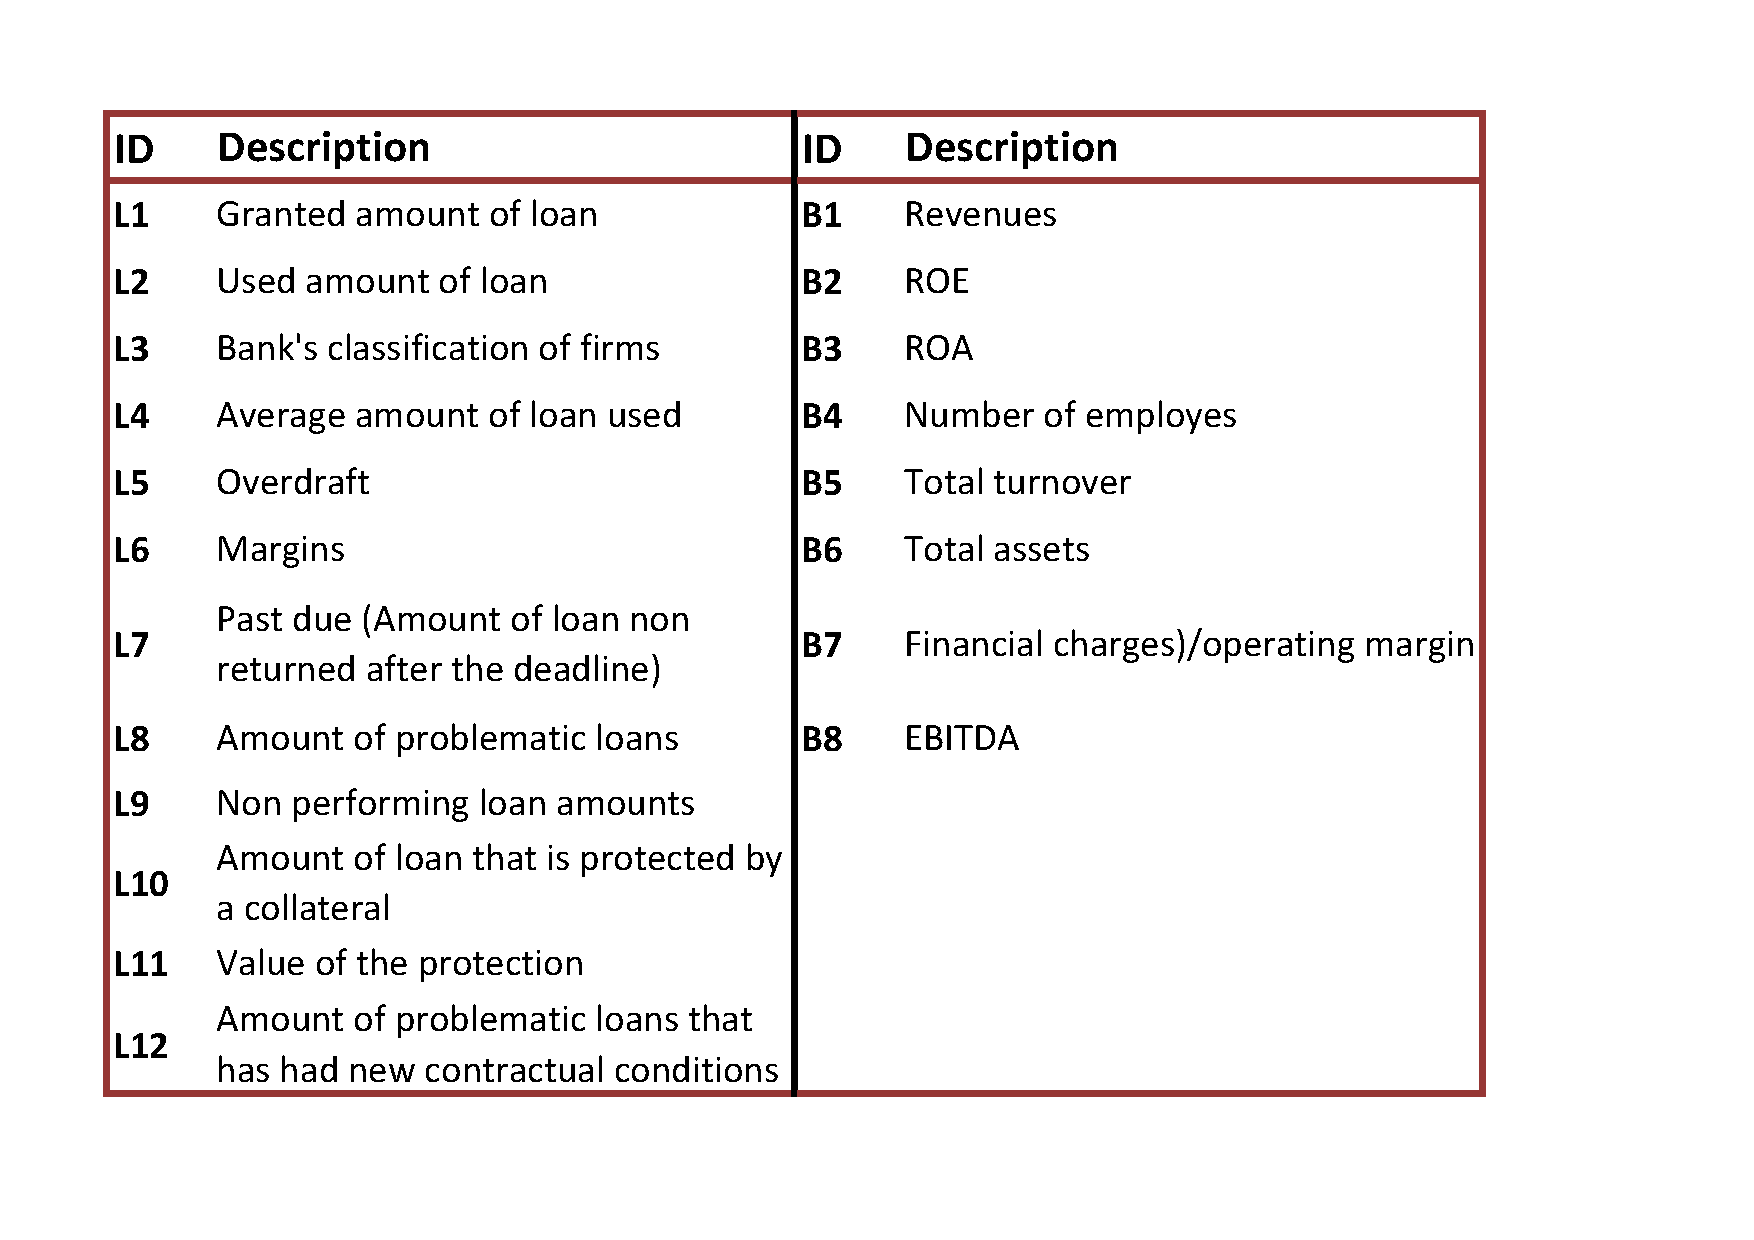
\includegraphics[width=180mm, height=80mm]{figs/Cdataset.pdf}
\caption{Loan dataset (L) and Balance sheet dataset (B): main
attributes. Loans data are quarterly from 2009 to 2014;
Balance sheet data have annual frequency from 2006 to 2014}
\end{figure}


\paragraph{The Balance sheet dataset.}



With the aim of improving the forecasts of the default status of Italian
firms, we have also performed some classification attempts  by
integrating credit information with some balance sheet indicator for Italian
companies. In particular, we used a set of firms balance sheet
indicators from the CEBI dataset: some important indicators are used
that are very similar to those used by Altman
\cite{altman-bankruptcy-17} also  in his famous Z-score. Among the
fundamental ones are those regarding the profitability of companies, as
in the case of ROE and ROA. The balance sheet dataset contains data
related to about 300,000 Italian firms; these are generally medium and
large companies. For each firms we used a set of eight indicators shown
in the Table. Balance sheet data are public data.\\
The three hundred thousand companies for which balance sheet data are available constitute a sub-sample of those belonging to the loan dataset. Therefore the dataset that uses both information on loans and balance sheet info is made up of about 300,000 companies.







